\chapter{基于传统视觉算法的无人机目标跟踪方法研究}


\section{引言}
针对目标检测问题,很多学者提出了不同的解决方法,但目标实时监测问题中的所涉及的目标尺度变化、被遮挡和实时性等问题仍然没有得到有效解决。本章针对无人机自主降落过程中的目标跟踪问题进行进一步分析,并提出了满足实时性需求的目标跟踪算法。

\section{目标跟踪问题的概述}

\begin{algorithm2e}[H]
	\SetAlgoLined
%	\KwData{this text}
%	\KwResult{how to write algorithm with \LaTeX2e }
	\BlankLine
	\SetKwInOut{Input}{Input}
	\SetKwFunction{Track}{Track}
	\SetKwFunction{Update}{Update}
	\SetKwFunction{Initialization}{Initialization}
	\Input{Image sequence $I_1, ..., I_T$ with bounding box $b_1$}
	\Initialization($I_1$, $b_1$)\;
	\For{$i=2$ \KwTo $T$}{
		$b_i\ \leftarrow$ \Track{$I_i$}\;
		$b_i\ \leftarrow$ \Update($b_t$, $b_{t-1}$, ..., $b_1$) \;
	}
	\caption{One-shot 目标跟踪算法}
\end{algorithm2e}


\section{形态学滤波方法进行图像预处理}

形态学滤波(Morphological Filtering)方法是一组非线性图像运算算子。该系列算子主要包括腐蚀(Erode)、膨胀(Dilate)、开运算(Opening)和闭运算(Closing)四种基本运算。在此四种运算的基础之上,一般还可以拓展出边缘提取、凸包运算、连通区域标记等复杂运算。通常而言,由于上述算子主要通过像素之间位置,形态学处理的对象为二值图像。

在有人机的感知规避领域,机载雷达是应用最为广泛的周边环境的感知器。除此之外,安装在机身各个位置的摄像头也是感知飞行器周边环境的重要传感器。一般而言,这些摄像头主要用于在空中识别周边的其他飞行器。由于民航飞行器的空间间隔一般较大,飞行器的成像尺寸一般较小,传统的预处理方法容易将这类小型目标当做噪声忽略。2011年,卡内基梅隆大学的三位学者使用形态学滤波方法对微小无人机检测的图像进行预处理\cite{dey2011cascaded},这篇文章图像预处理和图像检测的研究背景与本文的背景类似。
\begin{figure}[htb]   
	\centering
	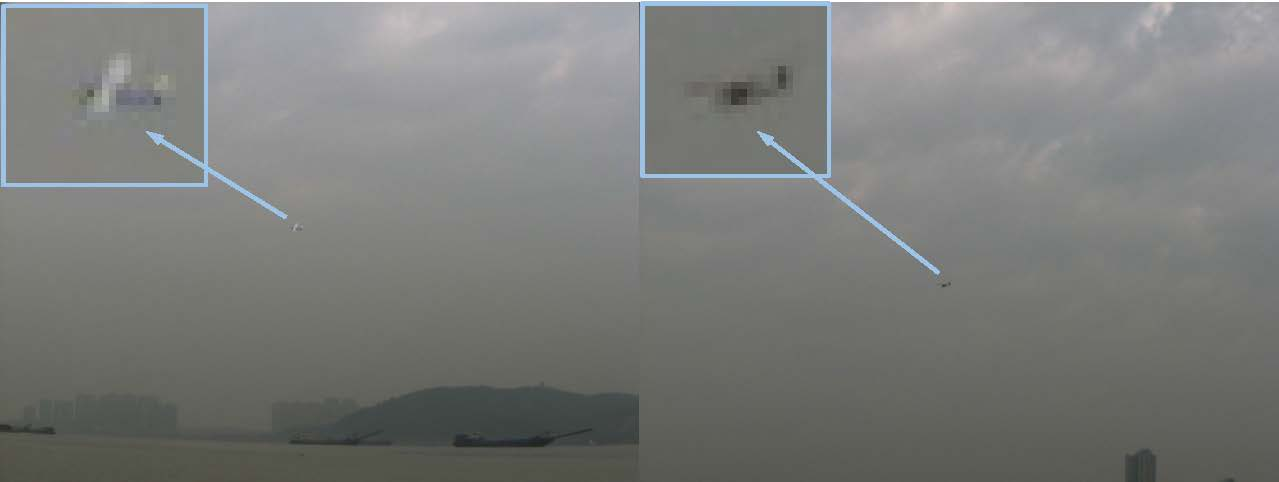
\includegraphics[width=\textwidth]{figs/chp03/01_small_uav_light_black.pdf}
	\caption{小型无人机$400\ m$在可见光相机成像效果}
	\label{fig:01_small_uav_light_black}
\end{figure}

针对本文涉及到的无人机目标识别问题,形态学滤波对图像预处理仍然是一种较为理想的方法。无人机距离摄像机较远的位置,由于机翼颜色和光照的影响,无人机的成像一般为一个亮点或一个暗点。对于试验中使用的白色无人机而言,在一次降落过程中,该无人机在距离摄像机$400\ m$左右的距离时,其成像效果如图\ref{fig:01_small_uav_light_black}所示。图中左上侧的矩形框是无人机目标放大后的结果。通过成像结果可以看到,左侧图像为无人机在转弯时,由于机翼为白色且面积较大,因此成像为一个白色为主的亮斑;右侧图像是无人机转弯完成后,无人机侧面虽然仍为白色,但由于反光面积相对较小,所以在相机中的成像为黑色为主的亮斑。


对于试验中使用的中等型号的无人机而言,其在距离摄像机$800\ m$左右的距离时,其成像效果如图\ref{fig:02_big_uav_light_black}所示。通过比较两种型号无人机的成像特性,本文设计将开运算与闭运算处理结果相减作为预处理的结果,主要针对小型无人机出现的白色和黑色亮斑变化情况进行处理。

\begin{figure}[htb]   
	\centering
	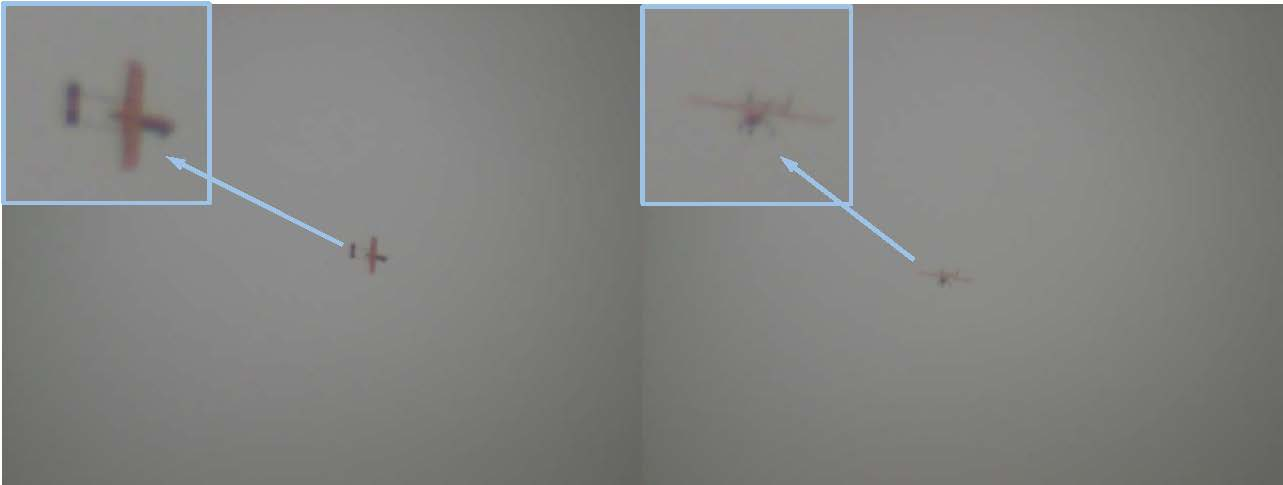
\includegraphics[width=\textwidth]{figs/chp03/02_big_uav_light_black.pdf}
	\caption{中型无人机$800\ m$在可见光相机成像效果}
	\label{fig:02_big_uav_light_black}
\end{figure}

开运算的特点是先进行腐蚀运算,再进行膨胀运算,能够消除细小物体,突出物体边缘,即亮出的区域增大。闭运算的特点是先进行膨胀运算,再进行腐蚀运算,能够消除细小空洞,使得临近的物体相互连通,即暗处的区域增大。为了利用开运算和闭运算结果的优点,该滤波方法的基本框架如图\ref{fig:04_morphogolical_method}所示。在Ubuntu环境下使用Python实现上述预处理算法,开运算和闭运算分别对每一帧图像($640 \times 480$)进行处理时间为$0.009\ s$至$0.013\ s$,整体时间消耗约为$0.016\ s$。

\begin{figure}[htb]   
	\centering
	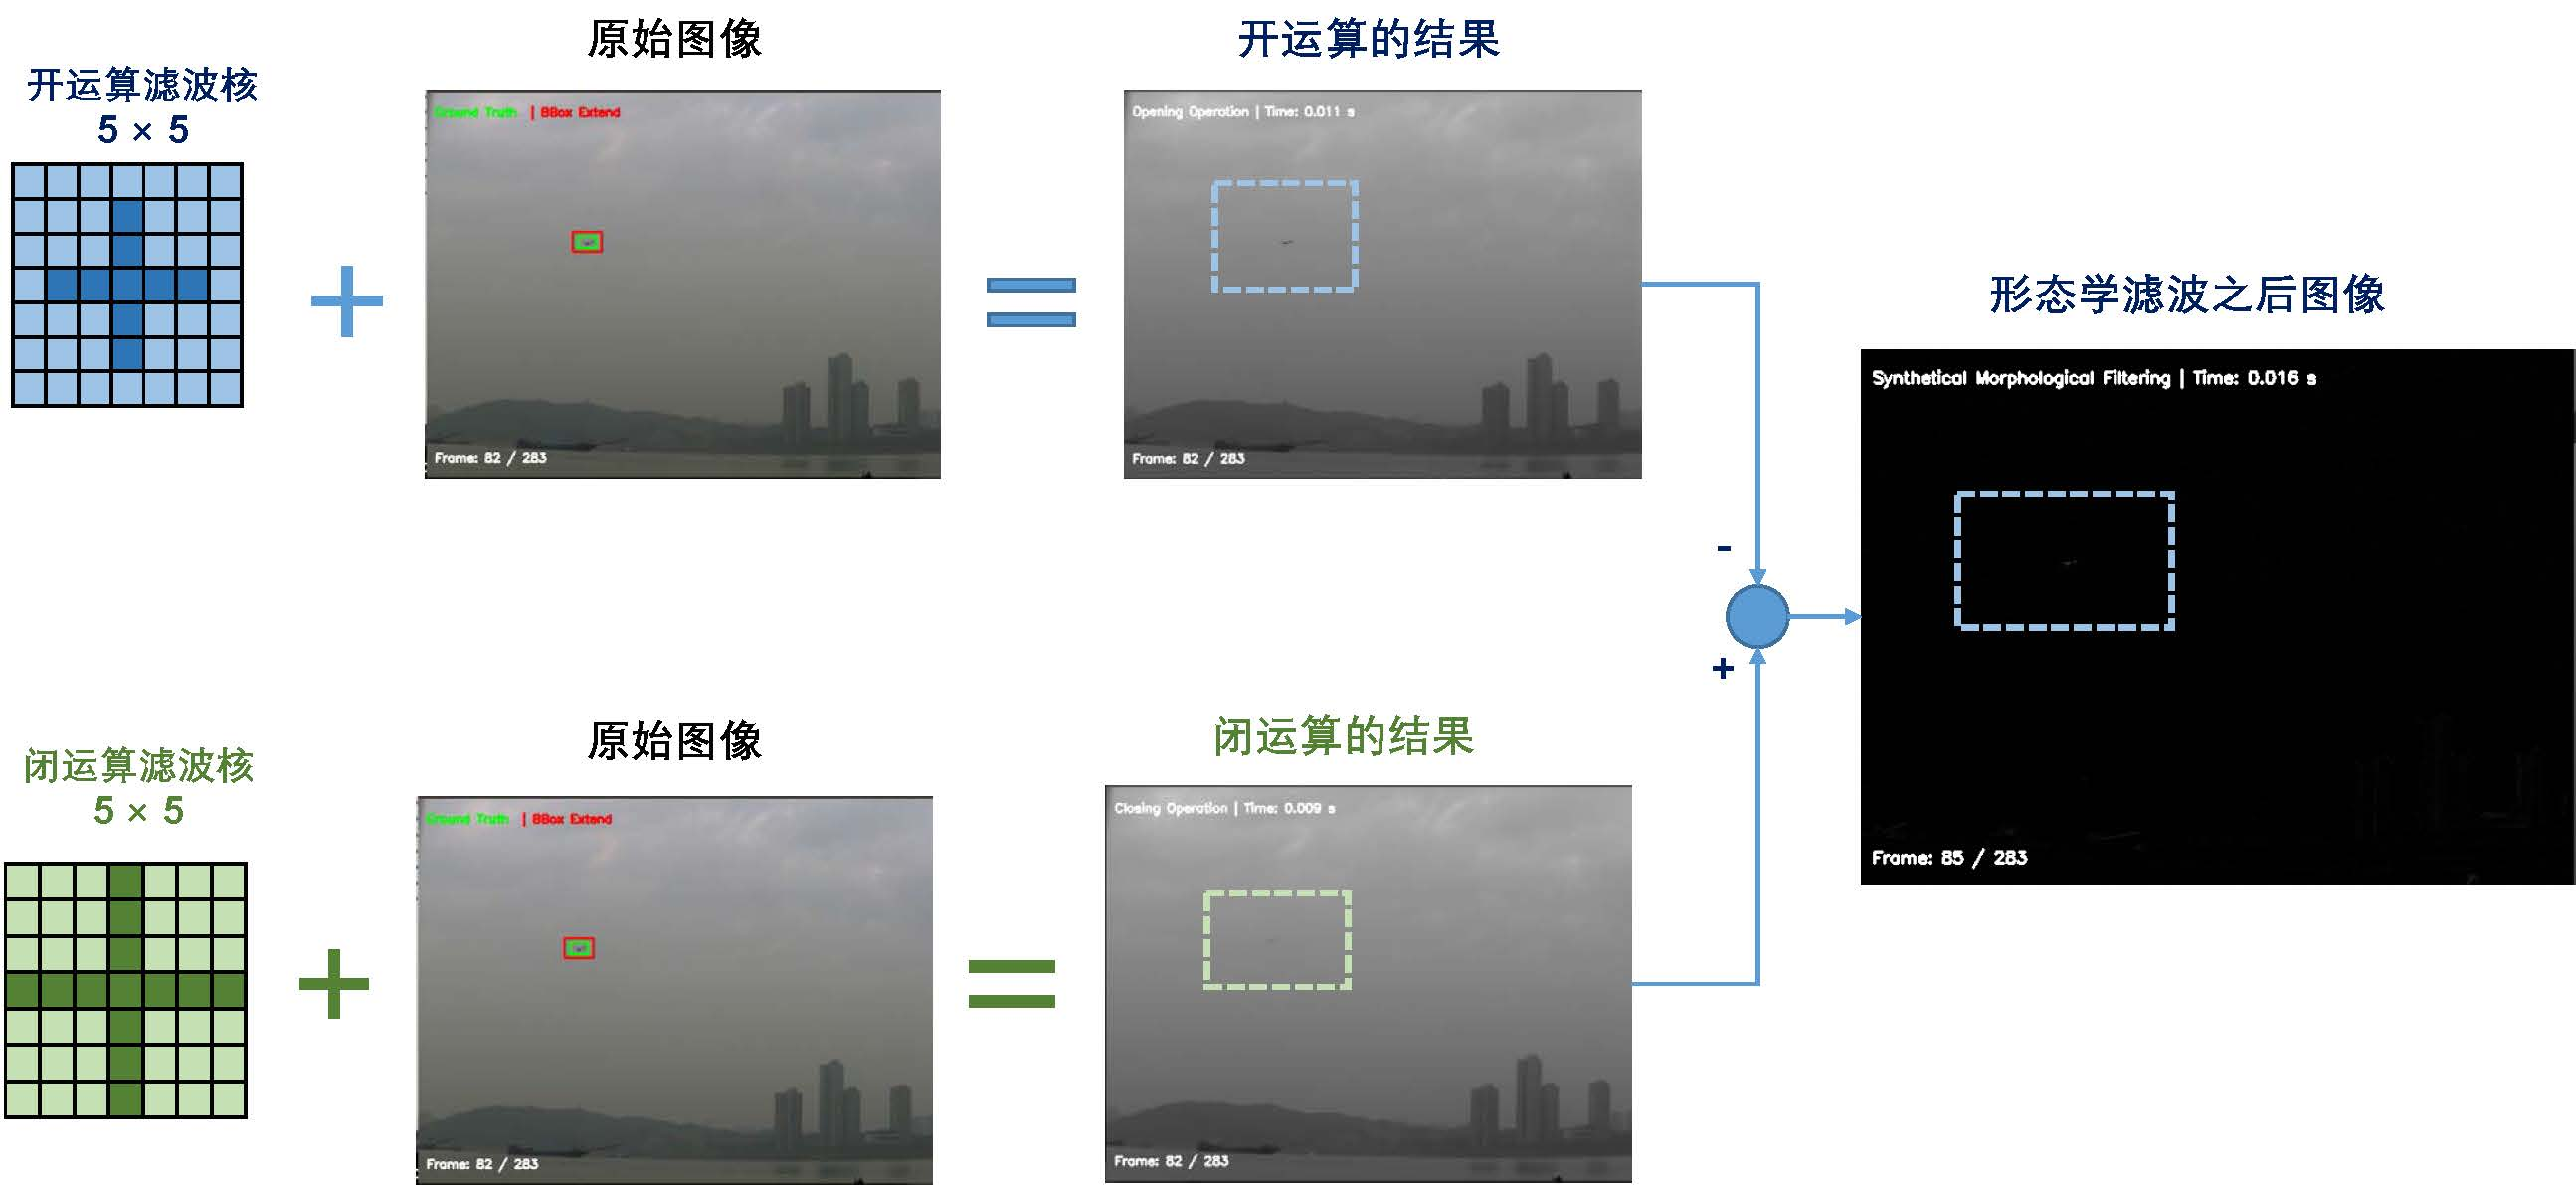
\includegraphics[width=\textwidth]{figs/chp03/04_morphogolical_method.pdf}
	\caption{形态学滤波预处理框架}
	\label{fig:04_morphogolical_method}
\end{figure}

将该算法运用到图\ref{fig:01_small_uav_light_black}中所示的图像,预处理之后的结果如图\ref{fig:03_small_uav_with_morphological}所示。结果表明,闭运算的结果减去开运算的结果能够将暗处和亮出的区域均进行筛选和保留,进一步突出小型无人机在远端时的图像特征,为后续的目标跟踪问题打下良好基础。

\begin{figure}[htb]   
	\centering
	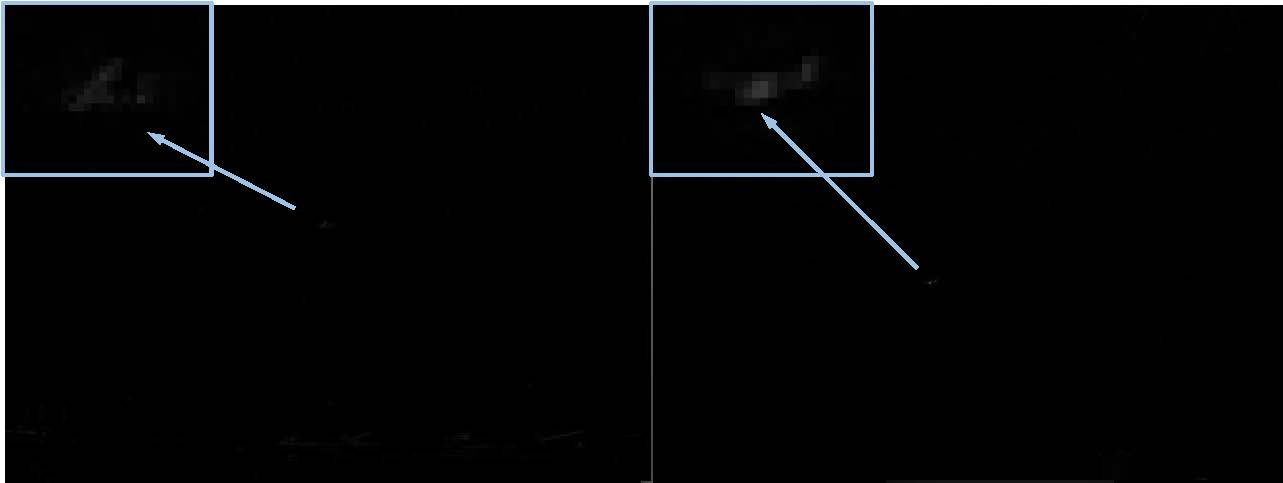
\includegraphics[width=\textwidth]{figs/chp03/03_small_uav_with_morphological.pdf}
	\caption{小型无人机在两种状态下使用形态学滤波处理之后的结果}
	\label{fig:03_small_uav_with_morphological}
\end{figure}


\section{基于角点检测的目标跟踪方法研究}





\section{基于主动态轮廓线的轮廓线的目标跟踪方法研究}






\section{基于Tracking-Learning-Detection的目标跟踪方法研究}
\subsection{Tracking-Learning-Detection基本框架}
TLD(Tracking-Learning-Detection)是一种针对单一目标的长时间跟踪算法(long-term tracking)。对于一段长时间的视频,我们希望对其中某个目标进行跟踪(一个人,一辆车,或者仅仅是一块运动的区域),首先在某一帧画面规定一个矩形框,框住的区域就是我们关注的目标,那么该算法做的事就是在接下来的视频中不断跟踪这个目标,无论该物体是否暂时离开画面,或者被遮挡,或者发生形变,都不会影响继续的跟踪。该框架包含这样三个部分:
\begin{itemize}
	\item 1. 跟踪器(Tracker),通过连续帧图像来预估所追踪对象的运动,这里假设帧与帧之间目标的相对运动有限,并且追踪目标保持在图像中始终可见。追踪器可能会出现追踪失败的情形,并且在目标跳出相机视野后无法恢复追踪。
	\item 2. 检测器(Detector),将各帧图像视为独立,并对每一帧图像都进行全扫面,以找出图像中所有与目标外貌相似的候选样本。该探测器会产生两类错误:错误的正样本(False Positives)和错误的负样本(False Negatives)。
	\item 3. 学习(Learning),学习过程实时观测追踪器和探测器的执行,并预估探测器的错误,生成训练样例以使能在未来避免类似的错误。学习组件假设追踪器和探测器都有可能出现失败执行,但学习组件的引入可以使得探测器生成更多的追踪目标外观,以区别背景。
\end{itemize}
\subsection{跟踪器的设计}
\subsubsection{前向后向传播算法}

\subsection{检测器的设计}
将各帧图像视为独立,并对每一帧图像都进行全扫面,以找出图像中所有与目标外貌相似的候选样本,候选样本的生成来自学习模块。该探测器会产生两类错误:错误的正样本(false positives)和错误的负样本(false negatives)。

\subsubsection{检测区域的生成}
检首先介绍一下基本的检测区域的生成和选择,即扫描窗网格。我们通过以下参数生成所有可能比例(scales)和转移(shifts)的初始边界框:比例step=1.2,水平step=10(百分比宽度),竖直step=10(百分比高度),最小边界框大小为20像素。针对一个图像(240*320)们可以生成约50K个边界框,准确数字需要基于初始边界框的宽高比。

\subsubsection{正样本区域的放射变换}
对每个正样本区域,进行$±1\%$范围的偏移,$±1\%$范围的尺度变化,$±10\%$范围的平面内旋转,并且在每个像素上增加方差为5的高斯噪声(确切的大小是在指定的范围内随机选择的),那么每个box都进行20次这种几何变换,那么10个box将产生200个仿射变换的bounding box,作为正样本。

\subsubsection{级联分类器的设计}
是由三个串行级联的三个部分组成,即级联分类器(Cascaded Classifier)。由于需要评估的边界框数量较多,每个单独的片段分类过程需要做到十分高效。如下图所示,我们将分类设计为三个阶段:图像变化(patch variance)、总体分类(ensemble classifier)、最近邻(nearest neighbor)。每个阶段都对片段进行一定的筛选排除。
\begin{figure}[htb]   
	\centering
	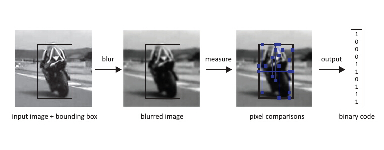
\includegraphics[width=\textwidth]{figs/161002_Thesis_Tracking_Section_04.pdf}
	\caption{集成分类器示意图}
	\label{fig:161002_Thesis_Tracking_Section_04}
\end{figure}

Patch Variance: 首先利用积分图求出当前要分类扫描窗的灰度值期望,再根据期望计算出方差,与原bounding-box的方差作对比,方差小于bounding-box方差的$50\%$的扫描窗都不会通过这个分类器。(这里的阈值是可以调整的)

集成分类器(Ensemble Classifier) 主要采用随机森林(Random Forest )的方法,其中特征选择2bitBP和Pixel Comparisions特征。Pixel Comparisons 的实现方法如下:首先,图像与高斯核进行方差为3像素的卷积,以提高转换稳健性和图像噪声。然后,根据决策树方法进行比较。


Random Forest 方法 :andom Forests方法主要源于BinaryDecision Trees。传统的决策树主要由一系列子二叉树组成,在每一个节点通过简单的YES/NO问题进行分类。在叶子节点,表明数据所属的类型。因此,对于一个决策树而言,一组特征数据通过不同节点的判断,最终得到一个分类结果。通过训练,我们可以根据训练数据的特征,构建一棵“完美”的决策树用于实际应用。但一般而言,单棵决策树训练速度较快,可以快速处理大量数据,但存在过拟合现象,在实际应用中误差较大。为解决单棵决策树存在的缺陷,1995年Ho以及2001年Breiman分别提出采用多个决策树并引入随机特征方法,即Random Forests。其中,通过构建相互独立的多个决策树,从而提高数据处理的多样性;通过在学习过程中引入随机性,来增强系统的鲁棒性。最后,根据少数服从多数的投票原则,判定一个数据的类别。

对样本的处理。Bootstrap Sampling 思想。通过有重复的随机抽取样本,重新组成新的样本集。原始数据集的数学表示如下:
$$\mathbf{\{Dat}{{\mathbf{a}}_{\mathbf{1}}}\mathbf{,Dat}{{\mathbf{a}}_{\mathbf{2}}}\mathbf{,Dat}{{\mathbf{a}}_{\mathbf{3}}}\mathbf{,Dat}{{\mathbf{a}}_{\mathbf{4}}}\mathbf{,Dat}{{\mathbf{a}}_{\mathbf{5}}}\mathbf{,Dat}{{\mathbf{a}}_{\mathbf{6}}}\mathbf{,Dat}{{\mathbf{a}}_{\mathbf{7}}}\mathbf{,Dat}{{\mathbf{a}}_{\mathbf{8}}}\mathbf{,Dat}{{\mathbf{a}}_{\mathbf{9}}}\mathbf{,Dat}{{\mathbf{a}}_{\mathbf{10}}}\mathbf{\}}$$

随机抽取之后的数据集如下:
$$\mathbf{\{Dat}{{\mathbf{a}}_{\mathbf{7}}}\mathbf{,Dat}{{\mathbf{a}}_{\mathbf{6}}}\mathbf{,Dat}{{\mathbf{a}}_{\mathbf{3}}}\mathbf{,Dat}{{\mathbf{a}}_{\mathbf{1}}}\mathbf{,Dat}{{\mathbf{a}}_{\mathbf{1}}}\mathbf{,Dat}{{\mathbf{a}}_{\mathbf{8}}}\mathbf{,Dat}{{\mathbf{a}}_{\mathbf{7}}}\mathbf{,Dat}{{\mathbf{a}}_{\mathbf{2}}}\mathbf{,Dat}{{\mathbf{a}}_{\mathbf{9}}}\mathbf{,Dat}{{\mathbf{a}}_{\mathbf{5}}}\mathbf{\}}$$

可以看到,则随机抽取之后的数据样本集中,不仅样本集的顺序发生了改变,个别样本集也出现了重复。

子特征集的提取。系统不再对全部特征进行训练,而是从中随机选出一个子集进行训练,基于这些子集得到不同类型的决策树。


Random Fern 方法:Random Fern 的思想就是用多个特征组合来表达对象。


\begin{figure}[htb]   
	\centering
	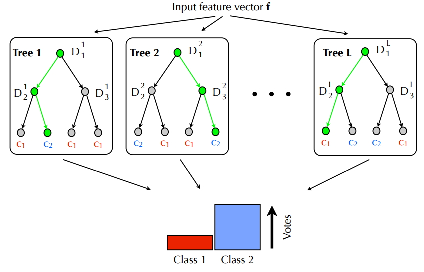
\includegraphics[width=\textwidth]{figs/161002_Thesis_Tracking_Section_05.pdf}
	\caption{集成分类器示意图}
	\label{fig:161002_Thesis_Tracking_Section_05}
\end{figure}

Random Fern 方法基于贝叶斯理论,主要是对简单贝叶斯分类器(Navie Bayes Classifiers)的改进。对于不同的特征$(f_1, f_2, ..., f_N)$而言,分类的最大化这些特征的后验概率:

$$\arg \max_{k}P(C_k|f_1, f_2, ..., f_N)$$

通过贝叶斯公式可以转换为求解最大化极大似然函数与先验概率的乘积

$$\arg \max_{k}P(f_1, f_2, ..., f_N|C_k)P(C_k)$$

这里引入各个特征相互独立的基本假设,方程可以将极大似然函数的求解进一步化简为
$$
P(f_1, f_2, ..., f_N|C_k)=\prod\limits_{i=1}^{N}P(f_i|C_k)
$$
此时,可以得到新的分类公式
$$
\arg\max_kP(C_k)\prod\limits_{i=1}^{N}P(f_i|C_k)
$$
但是在实际问题的求解过程中,每个特征的独立性假设过于严格,因此2007年的CVPR M.Oezuysal中提出Semi-Navie Bayes方法,即将特征进行分组,认为组与组之间保持严格的独立性,而组件的特征相互依赖。假设所有的特征可以分为$L$个组别,每个组别中包含$S$个特征,每个组别被称为Ferns,每一个特征组的表达为
$$
\mathbf{F}_l=\{f_{l,1}, f_{l,2},..., f_{l,S}\}
$$
为了在检测过程中计算便捷,选用二维编码的方式对图像进行描述,因此每一个特征满足$f_n\in\{{0,1}\}$。由此,可以进一步将极大似然函数重新表达
$$
P(f_1, f_2, ..., f_N|C_k)=\prod\limits_{i=1}^{L}P(\mathbf{F}_l|C_k)
$$
基于特征分组的分类公示为
$$
\arg\max_kP(C_k)\prod\limits_{i=1}^{L}P(\mathbf{F}_i|C_k)
$$
在实际训练过程中,由于训练样本数量较少,会导致分类概率为零的情况。因此,我们认为$P(\mathbf{F}|C_k)$符合Dirchlet分布,因此设定一个最小的概率输出
$$
p(\mathbf{F}=z|C_k)=\frac{\mathbb{N}(\mathbf{F}=z|C_k)+1}{\sum_{z=0}^{2^S-1}(\mathbb{N}(\mathbf{F}=z|C_k)+1)}
$$
其中,$\mathbb{N}(\mathbf{F}=z|C_k)$是计算在类别$C_k$情况下,观测到$\mathbf{F}=z$的特征个数。

\subsection{学习器的设计}
学习模块(Leaner)学习过程实时观测追踪器和探测器的执行,并预估探测器的错误,生成训练样例以使能在未来避免类似的错误。学习组件假设追踪器和探测器都有可能出现失败执行,但学习组件的引入可以使得探测器生成更多的追踪目标外观(generalizes to more object appearances),以区别背景。

PN学习即PN learning, P指代Positive Constraint,也称之为P-expert或者growing event,N指代Negative Constraint,也称之为N-expert或者pruning event。

P-expert的作用是发现目标的新的外观(形变),并以此来增加正样本的数量,从而使得检测模块更具鲁棒性;N-expert的作用是生成负的训练样本。N-expert的前提假设是,(被跟踪的)前景目标仅可能出现在视频帧中的一个位置,因此,如果前景目标的位置是确定的,那么其周围必然是负样例。

TLD模块中的PN学习作用是通过对视频序列的在线处理来逐步改善检测模块(TLD中的Detection)的性能。对视频中的每一帧而言,我们希望评估检测模块在当前帧中的误检,并以此来更新目标模型,从而使得在以后的视频帧处理过程中避免类似的错误再次发生。PN学习的关键在于两种类型的“专家(experts)”:P-experts检查那些被检测模块错误分类为正样本(前景目标)的数据;N-experts检查哪些被检测模块错误分类为负样本(背景)的数据;需要提醒的是,无论P-experts还是N-experts都会产生一定的偏差。那么,如果用这些存在偏差的数据来更新检测模块(目标模型),是否会造成检测模型的性能恶化呢?作者经过研究发现,尽管存在误差,在一定条件下,误差是允许的,并且检测模块的性能会因此得到改善。

PN学习包含四个部分:(1)一个待学习的分类器;(2)训练样本集–一些已知类别标签的样本;(3)监督学习–一种从训练样本集中训练分类器的方法;(4)P-N experts–在学习过程中用于产生正(训练)样本和负(训练)样本的表达函数;这四个部分之间的关系如下图所示:

首先根据一些已有类别标记的样本,借助监督学习方法来训练,从而得到一个初始分类器。之后,通过迭代学习,利用上一次迭代得到的分类器对所有的未赋予标签的样本数据进行分类,而P-N experts则找出那些错误分类的样本,并依此来对训练样本集做出修正,使得下一次迭代训练之后得到的分类器的性能有所改善。P-experts将那些被分类器标记为负样本,但根据结构性约束条件应该为正样本的那些样本赋予“正”的标签,并添加到训练样本集中;而N-experts则将那些被分类器标记为正样本,但根据结构性约束条件应该为负样本的那些样本赋予“负”的标签,并添加到训练样本集当中;这也就意味着,P-experts增加了分类器的鲁棒性,而N-experts则增加了分类器的判别能力。

每一个扫描窗口就表示一个图像片(image patch),图像片的类别标签用(b)(c)中的彩色圆点来表示。检测模块对每个图像片的类别赋值过程是彼此独立的,因此,N个扫描窗口就存在个类别标签的组合。而(b)则显示了其中一种可能的类别标签形式,这种类别标签标明,待检测目标在一个视频帧中可能同时出现在好几个区域,并且,待检测目标在相邻视频帧之间的运动没有连续性(例如(b)中最前面的图像中右上角的红色圆点在后面的两个图像中均没有出现),显然,这种类别标签形式是错误的。相反,(c)所示的类别标签形式则显示,每个视频帧中,目标只可能出现在一个区域,并且,相邻视频帧之间检测到的目标区域是连续了,构成了一个目标的运动轨迹。这种性质,我们称之为“结构性”的。PN学习的关键就是找到这种结构性的数据,从而来判别检测模块所产生的错误标签。

上述例子表明:P-experts寻找视频序列中的时域上的结构性特征,并且假设目标是沿着轨迹线移动的,即,相邻帧之间的移动很小,且存在一定的相关性。P-experts记录目标在上一帧中的位置,并根据帧与帧之间的跟踪算法(这里采用的是LK光流法)来预测目标在当前帧中的位置。如果检测模块将跟踪算法预测到的目标在当前帧中的位置标记为负标签,那么P-experts就产生一个正的训练样本;N-experts寻找视频序列中的空间域上的结构性特征,并且假设目标在一个视频帧中只可能出现在一个位置。N-experts对检测模块在当前帧中的所有输出结果以及跟踪模块的输出结果进行分析,并找到具有最大可能性的那个区域。当前帧中所有目标可能出现的区域当中,如果某个区域同最大可能性区域之间没有重叠,就将其认定为负样本。另外,具有最大可能性的那个区域,被用于重新初始化跟踪模块。

\section{基于滤波方法的目标跟踪方法研究}
 
1. 基本要点

1.1 Hann Window

The Hann function is typically used as a window function in digital signal processing to select a subset of a series of samples in order to perform a Fourier transform or other calculations.

1.2 Correlation

- Ref: http://www.cnblogs.com/hanhuili/p/4266990.html


- Correlation Filters作为衡量信号相似度的方法被用于跟踪,主要用于rigid模板
- Cross-correlation $f \star g$的定义为

\begin{align}
\begin{array}{l} (f \star g)(\tau )\mathop  = \limits^{def} \int_{ - \infty }^\infty  {f*(t)g(t + \tau )dt} \\ (f \star g)(n)\mathop  = \limits^{def} \sum\limits_{ - \infty }^\infty  {f*[m]g(m + n)}  \end{array}
\end{align}

- 衡量两个函数在某个时刻τ的相似程度,如下图所示。

%![img](http://images.cnitblog.com/blog/714517/201502/040044238596444.png)

1.3 MOSSE

% Ref:http://www.cs.colostate.edu/~draper/papers/bolme_cvpr10.pdf


- 模板与滤波模板的互相关运算
\begin{align}
g=h\text{ }\otimes  f \qquad (2)
\end{align}

- $g$ 表示输出的响应图
- $h$ 表示滤波模板
- $f$ 表示输入图像

- 定义互相关函数的快速傅里叶变换,即计算费时的卷积运算转换为普通的点乘运算。
\begin{align}
\mathcal{F}(g) = \mathcal{F}(h\otimes f)={{\mathcal{F}(h)}^{*}}\odot \mathcal{F}(f )
\end{align}

- $\mathcal{F}$ 表示傅里叶变换
- $\odot$ 表示每个元素的点乘
- $h^*$ 表示函数 $h$ 的共轭
- 时间计算开销为$O(n\log n)$,其中$n$是图像中像素的个数

- 对H函数的求解。为表达方便,上式用新的符号标记为
\begin{align}
G=F\odot H^*
\end{align}
因为是对于每个元素的点乘,由此可以得到对$H^*$的解析解
\begin{align}
H^* = \frac{G}{F}
\end{align}

- 考虑到对跟踪目标区域周边$m$个区块进行搜索,因此设计目标函数为
\begin{align}
\underset{{{H}^{*}}}{\mathop{\min }}\,\sum\limits_{i=1}^{m}{|{{H}^{*}}\odot{{F}_{i}}-{{G}_{i}}{{|}^{2}}} \qquad (5)
\end{align}
即对每一个输入的图像$F_i$和实际输出$G_i$是在频域的运算结果,目标是寻找合适的滤波器$H$,使得该滤波器与输入图像进行互相关运算后的输出结果与实际输出结果之间的误差最小。在频率域中,每一个运算都作用在图像的每一个元素上,由此可得
\begin{align}
\underset{H_{w,v}^{*}}{\mathop{\min }}\,\sum\limits_{i=1}^{m}{|H_{w,v}^{*}{{F}_{w,v,i}}-{{G}_{w,v,i}}{{|}^{2}}}\qquad (6)
\end{align}
对目标函数求导,寻找解析解
\begin{align}
\begin{array}{l} \frac{\partial }{{\partial H_{w,v}^*}}\sum\limits_{i = 1}^m {(H_{w,v}^*{F_{w,v,i}} - {G_{w,v,i}}) \cdot } {(H_{w,v}^*{F_{w,v,i}} - {G_{w,v,i}})^{\rm{*}}}{\rm{ = }}0\\  \Rightarrow \frac{\partial }{{\partial H_{w,v}^*}}\sum\limits_{i = 1}^m {H_{w,v}^*{F_{w,v,i}} \cdot {H_{w,v}}F_{w,v,i}^{\rm{*}} - H_{w,v}^*{F_{w,v,i}}G_{w,v,i}^{\rm{*}} - {H_{w,v}}F_{w,v,i}^{\rm{*}}G_{w,v,i}^{}{\rm{ + }}{G_{w,v,i}}G_{w,v,i}^{\rm{*}}} {\rm{ = }}0\\  \Rightarrow \sum\limits_{i = 1}^m {{F_{w,v,i}} \cdot {H_{w,v}}F_{w,v,i}^{\rm{*}} - {F_{w,v,i}}G_{w,v,i}^{\rm{*}}} {\rm{ = }}0\\  \Rightarrow {H_{w,v}}{\rm{ = }}\frac{{\sum\limits_{i = 1}^m {{F_{w,v,i}}G_{w,v,i}^{\rm{*}}} }}{{\sum\limits_{i = 1}^m {{F_{w,v,i}}F_{w,v,i}^{\rm{*}}} }} \qquad (7) \end{array}
\end{align}
对每一个元素求解,可以得到最优$H^*$函数的解析表达形式:
\begin{align}
H^*\text{=}\frac{\sum\limits_{i=1}^{m}{{{F}_{i}}\odot G_{i}^{\text{*}}}}{\sum\limits_{i=1}^{m}{{{F}_{i}}\odot F_{i}^{\text{*}}}}\qquad (8)
\end{align}

- 设计线性更新方式,可以得到模板$H$的更新公式:
\begin{align}
{{H}_{t}}=(1-\eta ){{H}_{t-1}}+\eta H(t)\qquad (9)
\end{align}

- 在运算过程中,将模板$H$与 输入的图像$f$做相关运算,在得到的响应图中,将数值最大的点作为当前图像模板的所在位置。

- 一般而言,分子和分母分别进行更新
\begin{align}
H_t=\frac{A_t}{B_t}\\
A_t=\mu F_t\odot G_t^*+(1-\mu)A_{t-1}\\
B_t=\mu F_t\odot F_t^*+(1-\mu)B_{t-1}
\end{align}






1.4 Kernelized Correlation Filters

- Ref:An Experimental Survey on Correlation Filter-based Tracking
- 训练:  Input (F) *Gaussian ---> Kernel H
- 更新:  Input(Z) * Kernel H --IFFT--> response map y

1.4.1 Ridge Regression Problem

- 定义输入输出函数关系$f(\mathbf{x}_i)=y_i$,即对于每一个输入$\mathbf{x}_i$都可以得到一个标签输出$y_i$,训练过程可以用最小化下列公式表达:
\begin{align}
\min_\mathbf{w}=\sum_{i}L(f(\mathbf{w},\mathbf{x}_i),y_i)+\lambda||\mathbf{w}||^2
\end{align}

- 其中,$\mathbf{w}$是对输入进行变换的参数,$\lambda$是正则化参数,避免目标方程过拟合,$L(\cdot)$是损失函数,可以根据需要进行设计。

- 在SVM中,损失函数定义为 Hinge 损失,即$L(f(\mathbf{w},\mathbf{x}_i),y_i)=\max (0,1-y_i f(\mathbf{w},\mathbf{x}_i))^2$

- 在Ridge回归中,损失函数的定义为二次损失,即

$L(f(\mathbf{w},\mathbf{x}_i),y_i)=(y_i-f(\mathbf{w},\mathbf{x}_i))^2$

- 如果函数$f(\cdot)$是对输入数据的线性变化,则可以得到解析解
\begin{align}
\mathbf{w}=(X^TX+\lambda I)^{-1}X^T\mathbf{y}
\end{align}
如果计算是在频域空间,则$X^T$需要变换为$X^H$,即$X^H=(X^*)^T$

- 如果函数$f(\cdot)$是非线性变换,即将输入数据$\mathbf{x}$转换到特征空间$\varphi(\mathbf{x})$,则参数$\mathbf{w}$定义为$\mathbf{w}=\sum_i\alpha_i \varphi(\mathbf{x}_i)$,由此可以得到
\begin{align}
f(\mathbf{x}_i)=\sum_{j=1}^n\alpha_i \kappa(\mathbf{x}_i,\mathbf{x}_j)
\end{align}
其中,$ \kappa(\mathbf{x}_i,\mathbf{x}_j)=<\varphi(\mathbf{x}_i), \varphi(\mathbf{x}_j)>$是核函数,定义$K$是核函数矩阵,即$K_{ij}=\kappa(\mathbf{x}_i,\mathbf{x}_j)$

此时目标函数的解为
\begin{align}
\mathbf{\alpha}=(K+\lambda I)^{-1}\mathbf{y}
\end{align}

- ​

​

1.4.2 引入循环矩阵求解目标函数

%- Ref: High-Speed Tracking with Kernelized Correlation Filters
%- http://blog.csdn.net/carrierlxksuper/article/details/46461245
% Code: 84.edge_box


- 引入循环矩阵的目的是产生一系列训练样本,从而可以简化计算量。

- 为避免计算矩阵求逆,引入循环矩阵求解。定义一组基采样(Base Sample)为$\mathbf{x}=(x_0, x_1, ..., x_{n-1})$,则循环矩阵的定义为
\begin{align}
X=C(\mathbf{x})=\begin{pmatrix}x_{0}&x_{1}&...&x_{n-1}\\x_{n-1}&x_{0}&...&x_{n-2}\\...&...&...&...\\x_{1}&x_{2}&...&x_{0}\end{pmatrix}
\end{align}
循环矩阵可以展开成如下形式
\begin{align}
X=F \mathtt{diag} (\mathcal{F(\mathbf{x})})F^H
\end{align}
其中$F$是傅里叶变换矩阵,即$\mathcal{F}(\mathbf{x})=\sqrt{n}F\mathbf{x}$。此时可以得到参数$\mathbf{w}$在时域的表达式为
\begin{align}
\mathbf{w}=F\mathtt{diag}(\frac{\mathcal{F}(\mathbf{x})}{\mathcal{F}(\mathbf{x})^*\odot\mathcal{F}(\mathbf{x})+\lambda})F^H\mathbf{y}
\end{align}
在频域的表达式为
\begin{align}
\mathcal{F}(\mathbf{w})=\frac{\mathcal{F}(\mathbf{x})\odot\mathcal{F}(\mathbf{y})}{\mathcal{F}(\mathbf{x})^*\odot\mathcal{F}(\mathbf{x})+\lambda}
\end{align}

- 进一步推导
\begin{align}
\mathbf{\alpha}=(K+\lambda I)^{-1}\mathbf{y}
\end{align}

- $\mathbf{k}^{\mathbf{xx}}$是核矩阵的第一行,即$K=C(\mathbf{k}^{\mathbf{xx}})$

- 引入核函数定义后,则Ridge回归对$\alpha$的求解公式变为
\begin{align}
\mathbf{\alpha}=(C(\mathbf{k}^{\mathbf{xx}})+\lambda I)^{-1}\mathbf{y}
\end{align}

\begin{align}
\mathbf{\alpha}=(F\mathtt{diag}(\mathcal{F}(\mathbf{k}^{\mathbf{xx}}))F^H+\lambda I)^{-1}\mathbf{y}
\end{align}

则在时域的解为

\begin{align}
\mathbf{\alpha}=\mathcal{F}^{-1}(\frac{\mathcal{F}(\mathbf{y})}{\mathcal{F}(\mathbf{k}^{\mathbf{xx}})+\lambda})
\end{align}

​

- 用一个核函数$\mathbf{k}$用于度量$\mathbf{x}$与$\mathbf{x'}$直接的关系,用符号$\mathbf{k}^{\mathbf{x}\mathbf{x'}}$表达

- 一个传统的多项式核函数$\mathbf{k}^{\mathbf{x}\mathbf{x'}}=(\mathbf{x}^T\mathbf{x'}+a)^b$可以表达为

\begin{align}
\mathbf{k}^{\mathbf{x}\mathbf{x'}}=(\mathcal{F}^{-1}(\mathcal{F}(\mathbf{x})^*\odot\mathcal{F}(\mathbf{x'}))+a)^b
\end{align}

- 一个传统的高斯核函数$\mathbf{k}^{\mathbf{x}\mathbf{x'}}=\exp{-\frac{1}{\sigma^2}(||\mathbf{x}-\mathbf{x'}||^2)}$可以表达为
\begin{align}
\mathbf{k}^{\mathbf{x}\mathbf{x'}}=\exp(-\frac{1}{\sigma^2}(||\mathbf{x}||^2+||\mathbf{x'}||^2-2\mathcal{F}^{-1}(\mathcal{F}(\mathbf{x})^*\odot\mathcal{F}(\mathbf{x'})))
\end{align}

- 在检测过程中,可以根据一个基本采用样本$\mathbf{x}$ 和新的采样$\mathbf{z}$得到的置信区域

根据回归方程的基本定义
\begin{align}
f(\mathbf{z})=\mathbf{w}^T\mathbf{z}=\sum_{j=1}^n\alpha_i \kappa(\mathbf{z},\mathbf{x}_j)
\end{align}

\begin{align}
f(\mathbf{z})=C(\mathbf{k}^{\mathbf{x}\mathbf{z}})^T\mathbf{\alpha}\\
f(\mathbf{z})=\mathcal{F}^{-1}(\mathcal{F}(\mathbf{k}^{\mathbf{x}\mathbf{z}})\odot\mathcal{F}(\mathbf{\alpha}))
\end{align}

其中$y$中数值最大的点的坐标为目标位置。

- 更新策略
\begin{align}
\mathcal{F}(\mathbf{\alpha})_t=\mu\frac{\mathcal{F}(\mathbf{z})}{\mathcal{F}(\mathbf{k})+\lambda}+(1-\mu)\mathcal{F}(\mathbf{\alpha})_{t-1}
\end{align}

\begin{align}
\mathcal{F}(\mathbf{k}_t)=\mu\mathcal{F}({\mathbf{k}^{\mathbf{x}\mathbf{z}}})+(1-\mu)\mathcal{F}(\mathbf{k}_{t-1})
\end{align}

​

​

1.5 引入概率来描述周边场景信息

- Ref: Fast Tracking via Spatio-Temporal Context Learning


- 一般而言,目标核心区域出现的信息是设计跟踪器的关键。但如果图像出现旋转和尺度变化,目标周边区域的图像信息同样可以作为有效信息进行处理。$\mathbf{x}^{*}\in \mathbb{R}^2$表示目标区域中心点所在位置,${{\Omega }_{c}}({{\mathbf{x}}^{*}})$ 表示在目标中心位置周边的图像区域,$\mathbf{z}$表示该区域中的一个像素点,$I(\mathbf{z})$表示该像素点对应的灰度值,$c(\mathbf{z})=(I(\mathbf{z}), \mathbf{z}))$表示在$\mathbf{z}$点的特征,${{X}^{c}}=\{\operatorname{c}(\mathbf{z})=(I(\mathbf{z}),\mathbf{z})|\mathbf{z}\in {{\Omega }_{c}}({{\mathbf{x}}^{*}})\}$ 表示在目标点周边场景(Context)所有像素点的集合。

- 定义$o$ 表示目标出现在当前区域,由此可以用目标出现的可能性可以用似然函数来描述
\begin{align}
c(\mathbf{x})=P(\mathbf{x}|o)
\end{align}
根据边缘联合概率的定义,可以将上式展开
\begin{align}
c(\mathbf{x})=\sum_{c(\mathbf{z})\in X^c}P(\mathbf{x}, c(\mathbf{z})|o))
\end{align}
根据条件概率公式,可以进一步得到

​
\begin{align}
c(\mathbf{x})=\sum_{c(\mathbf{z})\in X^c}P(\mathbf{x}|c(\mathbf{z}),o)P(c(\mathbf{z})|o)
\end{align}
​

- 设计一个与高斯函数形状类似的置信区间映射(Confident Map),即
\begin{align}
c(\mathbf{x})=b\exp(-|\frac{\mathbf{x}-\mathbf{x}^{*}}{\alpha}|)
\end{align}
由此可以得到在目标点周边任意像素的概率分布情况。

- 根据定义上下文先验可以根据灰度和权重函数相乘,来描述目标周边的表观信息
\begin{align}
P(c(\mathbf{z})|o))=I(\mathbf{z})\omega_\sigma(\mathbf{z}-\mathbf{x}^*)
\end{align}
权重函数的定义为一个高斯函数$\omega_{\sigma}(\mathbf{z})=a\exp(-\frac{|\mathbf{z}|}{\sigma^2})$

- 定义似然函数,用于描述目标周围区域信息与目标位置直接的模型
\begin{align}
P(\mathbf{x}|\operatorname{c}(\mathbf{z}),o)={{h}^{sc}}(\mathbf{x}-\mathbf{z})
\end{align}
其中${{h}^{sc}}(\mathbf{x}-\mathbf{z})$是目标位置与其周边场景中某一个点的相对距离和方向的度量,且不是一个对称函数。

- 根据置信区间映射的定义和全概率展开公式,可以得到
\begin{align}
b\exp(-|\frac{\mathbf{x}-\mathbf{x}^{*}}{\alpha}|)=\sum_{c(\mathbf{z})\in X^c}P(\mathbf{x}|c(\mathbf{z}),o)P(c(\mathbf{z})|o)\\
=\sum_{\mathbf{z}\in\Omega_c(\mathbf{x}^*)}{{h}^{sc}}(\mathbf{x}-\mathbf{z})I(\mathbf{z})\omega_\sigma(\mathbf{z}-\mathbf{x}^*)\\
=h^{sc}(\mathbf{x})\otimes (I(\mathbf{x})\omega_\sigma(\mathbf{x}-\mathbf{x}^*))
\end{align}

- 根据卷积定理求解似然函数,得到当前目标点的周边场景模型
\begin{align}
\mathcal{F}(b\exp(-|\frac{\mathbf{x}-\mathbf{x}^{*}}{\alpha}|))=\mathcal{F}(h^{sc}(\mathbf{x}))\odot\mathcal{F}(I(\mathbf{x})\omega_\sigma(\mathbf{x}-\mathbf{x}^*))
\end{align}

\begin{align}
h^{sc}(\mathbf{x})=\mathcal{F}^{-1}(\frac{\mathcal{F}(b\exp(-|\frac{\mathbf{x}-\mathbf{x}^{*}}{\alpha}|))}{\mathcal{F}(I(\mathbf{x})\omega_\sigma(\mathbf{x}-\mathbf{x}^*))})
\end{align}

- 利用该模型,可以得到在时序空间场景模型,定义其更新策略为线性模型
\begin{align}
H^{stc}_{t+1}=(1-\mu)H^{stc}_{t}+\mu h^{sc}_t
\end{align}

- 基于时序场景的模型,可以得到下一个时刻置信区间的更新
\begin{align}
c_{t+1}(\mathbf{x})=\mathcal{F}(h^{sc}_{t+1}(\mathbf{x}))\odot\mathcal{F}(I_{t+1}(\mathbf{x})\omega_{\sigma_{t}} (\mathbf{x}-\mathbf{x}^*_t))
\end{align}
​

- 此时建立目标函数,期寻找合适的$\mathbf{x}^*$使得置信区间的值最大
\begin{align}
\mathbf{x}^{*}_{t+1}=\arg\max_{\mathbf{x}\in \Omega_c(\mathbf{x}^*_t)}c_{t+1}(\mathbf{x})
\end{align}

- 根据连续两帧估计目标尺度变化的大小
\begin{align}
s_t^{'}=\sqrt{\frac{c_t(\mathbf{x}_t^*)}{c_{t-1}(\mathbf{x}_{t-1}^*)}}
\end{align}

- 根据过去一段时间,目标尺度的变化大小的平均值
\begin{align}
\bar{s}_t=\frac{1}{n}\sum_{i=1}^{n}s_{t-i}^{'}
\end{align}

- 下一个时刻目标尺度变化大小的计算
\begin{align}
s_{t+1}=(1-\lambda)s_t+\lambda\bar{s}_t
\end{align}

- 同时,更新权重函数参数$\sigma$
\begin{align}
\sigma{t+1}=s_t\sigma_t
\end{align}




1.5 局部跟踪

- Ref: [Real-time part-based visual tracking via adaptive correlation filters](http://blog.csdn.net/tjdatamining/article/details/45577295)

Ref: http://blog.csdn.net/tjdatamining/article/details/45577045


- 在图像$\mathbf{x}$位置,新观测图像$\mathbf{z}$置信分数的计算
\begin{align}
\hat{f}(\mathbf{z})=\mathcal{F}^{-1}(\mathcal{F}(\mathbf{k}^{\mathbf{x}\mathbf{z}})\odot\mathcal{F}(\mathbf{\alpha}))
\end{align}
​

- 联合置信度
\begin{align}
C^t=\sum_{i=1}^Nw_i^t\hat{f}^t_{p(i)}
\end{align}
其中,$\hat{f}^t_{p(i)}$表示在候选目标第$i$个区域的置信度,$p(i)$是局部响应的相关位置。

- PSR的定义

- 贝叶斯框架

- 观测到的置信图序列$O^t=[o^1, o^2, ..., o^n]$

- 描述物体仿射变换的参数$s^t$ 

- 最优的仿射参数$\hat{s}^t$可以通过极大后验进行计算
\begin{align}
\hat{s}^t=\arg\max_{s^t_j}p(s^t_j|O^t)
\end{align}

- 极大后验的计算可以转换为迭代求解
\begin{align}
p(s^t|O^t)\propto p(o^t|s^t)\int p(s^t|s^{t-1})p(s^{t-1}|O^{t-1})ds^{t-1}
\end{align}
其中$ p(o^t|s^t)$是当前时刻的观测的似然函数。此时,最大化该似然函数,就是最大化上式中的后验概率。这里设计该观测函数为
\begin{align}
p(o^t|s^t)=\frac{1}{|M^t|}\sum C^t(s^t)\odot M^t
\end{align}
其中$M^t$是一个空间约束模板(Spatial Layout Constraint Mask),该模板主要通过$N$各余弦函数窗口组成,使得靠近边缘的像素接近零。

- 一般来说,物体在连续两帧主要做布朗运动(Brownian Motion),则连续两个状态的模型可以用高斯分布来表达
\begin{align}
p(s^t|s^{t-1})=\mathcal{N}(s^t|s^{1:t-1},\Psi)
\end{align}
​

1.6 对尺度变换的处理

- MOSSE和KCF方法只针对固定大小的目标,即搜索窗口的大小是固定的。
- SAMF和DSST采用尺度池方法(Scaling Pool),在对输入的图像按一定尺寸进行切割,之后对每一个不同大小的图像进行后续运算。

1.7 DDST方法

%Ref: http://blog.csdn.net/roamer_nuptgczx/article/details/50134633

%Ref: http://blog.csdn.net/autocyz/article/details/48651013

%Ref HOG: https://xiangjiang.live/2016/02/09/histograms-of-oriented-gradients/

1.7.1 基本思想

- 核心是利用多个维度的特征来解决尺度变化问题
- 一维滤波器来估计目标的尺度变换
- (1 灰度 + 27 Hog)* 2D Hann Window
- 二维滤波器来估计目标的旋转变换
- Resize 固定尺寸33个
- 分别提取31D HOG 特征
- 级联成金字塔 33层 * 1D Hann Window
- 三位滤波器来估计目标尺度空间的位置变化

1.7.2 经典多维度特征互相关滤波方法

- 对于一副图像,我们使用$d$维特征来进行描述,定义在目标区域的一块图像的大小为$f$
- 对于不同维度的特征用$f^l\ l \in {1, 2, ..., d}$来表达

\begin{align}
\underset{{{H}^{*}}}{\mathop{\min }}\,\sum\limits_{l=1}^{d}{|{{H}^{*}}\odot{{F}^{l}}-{{G}^{l}}{{|}^{2}}}+\lambda \sum_{l=1}^{d}|H^{l}|^2
\end{align}

​	可以得到解析解
\begin{align}
H^l\text{=}\frac{\sum\limits_{i=1}^{m}{{{F}^{l}}\odot {G^{i}}^{{*}}}}{\sum\limits_{i=1}^{d}{{{F}^{i}}\odot {F^{i}}^{\text{*}}}+\lambda}=\frac{A^{l}_{t}}{B^{l}_{t}+\lambda}
\end{align}

- 更新策略

\begin{align}
A_t^l=(1-\mu)A_{t-1}^{l}+\mu G_{t}^{*}\odot F_{t}^{l}\\
B_t^l=(1-\mu)B_{t-1}^{l}+\mu \sum_{l=1}^{d}{F_{t}^{l}}^{*}\odot F_{t}^{l}\\
\end{align}

- 对目标检测的计算,即响应区域的计算

\begin{align}
\mathbf{y}_t=\mathcal{F}^{-1}(\frac{\sum_{i=1}^{d}{A^{l}_{t-1}}^*\odot Z^{l}_{t}}{B_{t-1}+\lambda})
\end{align}

1.7.3 基本流程

- 先利用二维Filter确定新位置

- 再用一维Filter精确估计目标的尺度变化

- 尺度选择原则

$a^nP_{t-1}\times a^nR_{t-1}\ n \in \{-\frac{S-1}{2},...,\frac{S-1}{2}\} $

- a = 1.02
- S = 33,即尺度滤波器的总尺度级数。

- 根据不同尺度缩放的比例,在原图中进行截取

- 将截取的图像缩放会同等比例 $scale_model_sz$ ,计算HOG特征

- 将HOG特征转换为1D向量

1.7.4 多尺度的处理

- 在目标区域提取$M\times N \times S$的立方体,其中$M$和$N$代表高和宽,$S$代表尺度等级。
- 构造一个三维高斯函数


- 计算互相关输出
\begin{align}
\mathbf{y}=\frac{\mathcal{F}^{-1}(\sum_{i=1}^{d}{A^{l}}^*\odot Z^{l})}{B+\lambda}
\end{align}




1.7.5 提速算法

- Sub-grid迭代求解互相关值
\begin{align}
\mathbf{y}_t=\mathcal{F}^{-1}(\frac{\sum_{i=1}^{d}{A^{l}_{t-1}}^*\odot Z^{l}_{t}}{B_{t-1}+\lambda})
\end{align}

- 在$Y_t$的高频位置采用Zero-Padding方法,使其尺寸等于Interpolation Grid

- 使得采样维度下降的方法

- 跟踪目标模板$u_t$的更新
\begin{align}
u_t = (1-\mu)u_{t-1}+\mu f_t
\end{align}

- $A_t^l$可以化简为
\begin{align}
A_t^l=G^* \mathcal{F}(u_t^l)
\end{align}

- 建立一个映射矩阵$P_t$,其维度大小是$\hat{d} \times d$,其中$\hat{d}$是压缩特征的维数。该矩阵的计算方式通过使构造误差最小得到,即最下化一下公式
\begin{align}
\epsilon=\sum_\mathbf{n}||u_t(\mathbf{n})-P_t^TP_tu_t(\mathbf{n})||^2
\end{align}
其中$\mathbf{n}$是在模板$u_t$中的一个元素。当映射矩阵满足$P_tP_t^T=I$时得到最优解,具体求解方式是对Auto-Correlation矩阵进行特征值分解
\begin{align}
C_t=\sum_{\mathbf{n}}u_t(\mathbf{n})u_t(\mathbf{n})^T
\end{align}
其中映射矩阵$P_t$的每一行是$C_t$矩阵的特征向量。

- 由此两个滤波器的计算可以作用在压缩之后的采样图像上

\begin{align}
\hat{F}_t=\mathcal{F}(P_tf_t)\\
\hat{U}_t=\mathcal{F}(P_tu_t)
\end{align}

- 使用压缩后的采样后,平移滤波器的数学表达为
\begin{equation}
\mathbf{y}_t={\mathcal{F}^{-1}}(\frac{\sum_{i=1}^{\hat{d}}{\hat{A}^{*l}_{t-1}} \odot \hat{Z}^{l}_{t}}{\hat{B}_{t-1}+\lambda})
\end{equation}
%\begin{align}
%\mathbf{y}_t=\mathcal{F}^{-1}(\frac{\sum_{i=1}^{\hat{d}}{\hat{A}^{l}_{t-1}}^*\odot \hat{Z}^{l}_{t}}{\hat{B}_{t-1}+\lambda})
%\end{align}
- 对尺度滤波器的压缩处理(见原文)
 1.7.6 思考
尺度变换只针对于整体缩放,是否有考虑横向和纵向不同尺寸的缩放?
1.8 对Filter和Loss Function的改进
- 原始目标函数
\begin{align}
\min_\mathbf{w}=\sum_{i}l(f(\mathbf{x}_i)-y_i)+\lambda||\mathbf{w}||^2_2
\end{align}
其中$f(\mathbf{x}_i)=\mathbf{w}^T\varphi(\mathbf{x}_i)$
- Loss Function可以改造为
\begin{align}
l \in \{l_1, l_1l_2, l_{2,1}\}
\end{align}
- Loss-1 允许误差巨大变化,能够忽略目标表观的显著变化
- Loss-1,2 对全局改变不敏感,能更在处理被遮挡和目标表观缓慢变化情况。
- Loss-2,1 能够处理局部表观变化的情况
- 原始目标函数是NP-hard问题,目标函数可以等价变换为
\begin{align}
\min_{\mathbf{w}\ \mathbf{e}}=\sum_{i}l(e_i)+\lambda||\mathbf{w}||^2_2\\
s.t.\ e_i=y_i - f(\mathbf{x}_i)
\end{align}
- $e_i$描述回归值与真实值之间的误差
- $y_i$是二维高斯函数
- 变换后的目标函数是凸函数
- 经过变换的函数仍然是一个NP-hard问题,因此只能通过迭代方法求解
\begin{align}
\min_{\mathbf{w}\ \mathbf{e}}=\sum_{i}(f(\mathbf{x}_i) + e_i - y_i)^2+\lambda||\mathbf{w}||^2_2 + \tau \sum_i l(e_i)\\
\end{align}
上述公式可以转化为两部分分别进行求解
\begin{align}
\min_{\mathbf{w}}||\mathbf{f}(\mathbf{X})+\mathbf{e}-\mathbf{y})||^2_2+\lambda||\mathbf{w}||^2_2\\
\min_{\mathbf{e}}||\mathbf{f}(\mathbf{X})+\mathbf{e}-\mathbf{y})||^2_2+\tau l(\mathbf{e})\\
\end{align}
其中,$\mathbf{X}$是采样矩阵,每一行代表一个采样。
- 对第一个的求解和传统方法一样
- 对第二个的求解需要根据不同损失函数进行设计
 2. 特征选择
- HOG特征基于每一个原包的梯度统计特性,局部鲁棒性强,但对目标发生形变是描述效果差。
- Color直方图基于全局统计,在一定程度上具有全局不变性。

\section{引入转台运动后的目标位置估计}
\subsection{低通滤波器的设计}
无人机的目标在像平面的投影通常是由多个像素点组成,上述目标识别算法主要通过求解所有像素点的几何平均位置来作为后续转台控制和无人机位置解算的输入。由于相机在成像过程中存在噪声扰动,所以图像识别之后的结果也会受到噪声的污染,因此本节设计一个低通滤波器对目标的位置和移动速度进行滤波。

一般情况,均认为系统的图像采样时间间隔基本相同。但通过实际测试实验发现系统采样时间抖动较大,其中一组降落过程中的图像采样时间间隔情况如图\ref{fig:chp04_01_delta_time_stamp}所示。图中的蓝色实线表明系统在最后18\ s左右的降落过程中,系统的采样出现较大的波动,其峰值甚至达到190\ ms。所以,在进行像平面位置估计等计算时,需要实时计算每一帧的采样时间间隔,以此来提升解算精度。

\begin{figure}[htb]   
	\centering
	\includegraphics[width=0.8\textwidth]{figs/chp04/chp04_01_delta_time_stamp.pdf}
	\caption{一组降落实验中的图像时间间隔采样情况}
	\label{fig:chp04_01_delta_time_stamp}
\end{figure}

定义目标的在像平面的坐标为$\mathbf{p}_{uav} = (u, v)^T$,经过低通滤波器之后的像平面坐标为$\bar{\mathbf{p}}_{uav} = (\bar{u}, \bar{v})^T$,目标点的移动速度定义为$\dot{\mathbf{p}}_{uav} = (\dot{u},\dot{v})^T$。根据低通滤波器的定义,可以得到目标原始位置坐标和滤波之后坐标之间的关系
\begin{align}
\mathbf{p}(s) = \frac{1}{\tau s+1}\bar{\mathbf{p}}
\end{align}
对上式微分可以得到速度与滤波之后坐标之间的关系
\begin{align}
\dot{\mathbf{p}}(s) = \frac{s}{\tau s+1}\bar{\mathbf{p}}
\end{align}
由于采样是离散系统,因此将上式进行双线性变换(Bilinear Transform)\cite{franklin1998digital},即将连续系统转换离散系统,通过下式进行变换
\begin{align}
s \mapsto \frac{2}{T_s}\frac{z-1}{z+1}
\end{align}
带入后可以得到
\begin{align}
\mathbf{p}[z] &= \frac{1}{\frac{2}{T_s}\frac{z-1}{z+1}}\bar{\mathbf{p}} \\
&= \frac{\frac{T_s}{2\tau+T_s}(z+1)}{z-\frac{2\tau-T_s}{2\tau+T_s}}\bar{\mathbf{p}}
\end{align}
和
\begin{align}
\dot{\mathbf{p}}[z] &= \frac{\frac{2}{T_s}\frac{z-1}{z+1}}{\frac{2}{T_s}\frac{z-1}{z+1}+1}\bar{\mathbf{p}} \\
&= \frac{\frac{2}{2\tau+T_s}(z-1)}{z-\frac{2\tau-T_s}{2\tau+T_s}}\bar{\mathbf{p}}
\end{align}
对上式两个公式进行逆z变换,可以得到求解期望位置的差分公式
\begin{align}
\mathbf{p}[n] = \frac{2\tau-T_s}{2\tau+T_s} \mathbf{p}[n-1]+ \frac{T_s}{2\tau+T_s}(\bar{\mathbf{p}}[n-1] + \bar{\mathbf{p}}[n-1] )
\end{align}
同理得到求解期望速度的差分公式为
\begin{align}
\dot{\mathbf{p}}[n] = \frac{2\tau-T_s}{2\tau+T_s}\dot{\mathbf{p}}[n-1]+ \frac{2}{2\tau+T_s}(\bar{\mathbf{p}}[n-1] - \bar{\mathbf{p}}[n-1] )
\end{align}
其中$\mathbf{p}[0] = \bar{\mathbf{p}}[0]$和$\dot{\mathbf{p}}[0] = 0$,$\tau$是滤波的阶段频率,$T_s$是每次采样时间间隔。


\subsection{引入转台信息后的位置估计}
由于受到采样间隔时间和转台系统误差的影响,转台在俯仰角和方位角的返回值同样存在较大偏差。左右两侧转台在一组降落过程中的末状态角度读取结果和偏差计算如图\ref{fig:chp04_02_pan_tilt_status}所示。其中,图中的蓝色虚线为通过串口读取到的转台实际角度,橙色实线为相邻两次采样之间转台的变化量。通过曲线的趋势可以看到,由于采样时间的波动,转台俯仰角和方位角的变化率整体平稳,在$12\ s$到$16\ s$之间,两个转台的俯仰角和横滚角都出现了较大的几次波动,这几次波动与图\ref{fig:chp04_01_delta_time_stamp}响应时刻的采样间隔变大相吻合。同时,突然出现的较大延时,还会对转台控制系统和目标在位置中的估计带来较大影响,因此不能仅仅依赖目标在图像中的位置来中下一帧的位置进行估计,而是需要通过读取转台的角度信息来对原有模型进行修正。
\begin{figure}[htb]   
	\centering
	\includegraphics[width=\textwidth]{figs/chp04/chp04_02_pan_tilt_status.pdf}
	\caption{时间采样间隔的对转台读数的影响情况}
	\label{fig:chp04_02_pan_tilt_status}
\end{figure}

在转台转动情况已知的情况下,如果目标相对于引导坐标系不动,则可以得到其在像平面的运动情况。定义$P_c$是目标点在相机坐标系的一点,$P_r$是目标点在引导坐标系的一点,两个坐标系之间的转换关系为
\begin{equation}
P_r = T_c P_c
\end{equation}
其中$T_c$是一个$4 \times 4$转换矩阵,将相机坐标系的一点转换为引导坐标系的一点。考虑到转台的转动情况定义当前时刻转换矩阵为$T_c(t)$,在相机坐标系的坐标为$P_c(t)$ 上一时刻的转换矩阵为$T_c(t-1)$,在相机坐标系的坐标为$P_c(t-1)$。在目标点相对于引导坐标系不变的情况下,该点的坐标系可以表示为
\begin{equation}
P_r = T_c(t) P_c(t) =T_c(t-1) P_c(t-1)
\end{equation}

通过变换可以得到
\begin{equation}
\label{eq:chp04_predict_position}
P_c(t-1) = T_c(t-1)^{-1}T_c(t) P_c(t)
\end{equation}

由于转台的读数可以获得,因此转换矩阵之间的关系可以表示为

\begin{equation}
T_c(t) = R_Y(\psi)R_X(\phi)T_c(t-1)
\end{equation}

同理可得
\begin{equation}
T_c(t-1)^{-1} = T_c(t)^{-1}R_Y(\psi)R_X(\phi)
\end{equation}

带入\ref{eq:chp04_predict_position}式之后,可以得到
\begin{equation}
P_c(t-1) =T_c(t)^{-1}R_Y(\psi)R_X(\phi)T_c(t) P_c(t)
\end{equation}

因为实验所用转台的最小转动角度为$0.006 \degree$,可以将转换矩阵的相关量进行近似求解
\begin{align}
&\cos \phi \approx \cos \psi \approx 1 \\
&\sin \phi \approx \phi \\
&\cos \psi \approx \psi \\
&\sin \phi \approx \sin \psi \approx 0 \\
\end{align}

如果初始状态,系统存在水平方向的偏差角度$\theta$,则此时的转换矩阵为
\begin{equation}
T_c(t) =\begin{pmatrix} 1 & 0 & 0 & 0 \\ 0 & \cos \theta & -\sin \theta & \rho_y \\0 & \sin \theta & \cos \theta & \rho_z \\ 0 & 0 & 0 &0 \end{pmatrix}
\end{equation}

\begin{equation}
T_c(t)^{-1} =\begin{pmatrix} 1 & 0 & 0 & 0 \\ 0 & \cos \theta & \sin \theta & -\cos \theta \rho_y -\sin \theta \rho_z \\0 & -\sin \theta & \cos \theta & \sin\theta \rho_y-\cos \theta \rho_z \\ 0 & 0 & 0 & 1 \end{pmatrix}
\end{equation}

带入上述公式之后,可以得到
\begin{align}
&X_{t-1} = X_t + \psi \sin \theta Y_t + \psi \cos \theta Z_t + \psi \rho_z \\
&Y_{t-1} = -\psi \sin \theta X_t +  Y_ t - \phi Z_t + \phi \sin \theta \rho_y - \phi \cos \theta \rho_z \\
&Z_{t-1}  = -\psi \cos \theta X_t + \phi  Y_ t + Z_t + \phi \cos \theta \rho_y - \phi \sin \theta \rho_z
\end{align}

根据相机的针孔成像模型
\begin{equation}
x = f \frac{X}{Z}
\end{equation}
则像素的向后递推公式为
\begin{align}
x_{t-1} = f\frac{x_t+\psi \sin \theta y_t + f\psi \cos \theta}{- \psi \cos \theta x_t + \phi y_t + f} \\
y_{t-1} = f\frac{-\psi \sin \theta x_t +y_t -f\phi}{- \psi \cos \theta x_t + \phi y_t + f} \\
\end{align}
当系统的初始偏差不存在时,向后地推公式可以表达为
\begin{align}
x_{t-1} = f\frac{x_t + f\psi }{- \psi  x_t  + \phi y_t + f} \\
y_{t-1} = f\frac{y_t -f\phi}{- \psi  x_t + \phi y_t + f}
\end{align}
同理,如果已知上一帧位置和转台转动的情况,可以推算出当前帧的像素位置
\begin{align}
x_{t} = f\frac{x_{t-1} - f\psi }{x_{t-1}  \psi  - \phi y_{t-1} + f} \\
y_{t} = f\frac{y_{t-1} -f\phi}{  x_{t-1} \psi - \phi y_{t-1} + f} \\
\end{align}

 



